\documentclass{article}
\usepackage[T1]{fontenc}
\usepackage[utf8]{inputenc}
\usepackage{amsmath}
\usepackage{amssymb}
\usepackage{hyperref}
\usepackage{parskip}
\usepackage{float}
\usepackage{graphicx}
\usepackage{listings}
\usepackage{cleveref}
\usepackage{circuitikz}
\usepackage{listings}

\title{Design of Digital systems 1 TFE4141 - Assignment 1}
\author{Sindre Hansen \and Laurits Telle Riple}
\date{Fall 2016}

\renewcommand\thesection{Q\arabic{section}}
\renewcommand\thesubsection{\thesection\alph{subsection}}

\begin{document}
\begin{figure}
  \centering
  
\includegraphics[width=0.5\textwidth]{images/logontnu_eng}
\end{figure}
\maketitle
\rule{\linewidth}{0.5mm}

\section{What is $01000_2 + 01001_2$?}
$01000_2 + 01001_2 = 10001_2 = 17 $

\section{Which number does $1111_2$ represent}
\subsection{In 4-bit unsigned format?}
$1111_2 = 15$
\subsection{In 4-bit signed format (2's complement)?}
To go from 2's complement to binary you invert every bit and add
one. Thus, $1111_2 \rightarrow 0000_2 \rightarrow 0001_2$

\section{What does ``Dynamic range'' in the context of number
  representation mean?}
Dynamic range is the ratio between the largest and smallest values
that a certain quantity can assume.

\section{What has highest dynamic range of a 32 bit floating point
  number and a 32 bit fixed point number?}
A floating point representation is similar to scientific notation,
where you have a significand and an exponent. This allows you to have
very large dynamic range.

Fixed point representation is less costly to implement than floating
point, but you get a much smaller range of numbers.

\section{How are floating point numbers and fixed point numbers spaced
  across the dynamic range?}
With floating point numbers the numbers that can be represented is not
uniformly spaced. They move further apart as the scale grows larger.

Fixed point numbers are evenly spaces across the range.

\section{Add the numbers from Q1 in the same way as taught in
  school.}
\begin{tabular}{c@{\,}c@{\,}c@{\,}c@{\,}c@{\,}c@{\,}}
  & $_1$\\
  & 0 & 1 & 0 & 0 & 0 \\
  + & 0 & 1 & 0 & 0 & 1 \\
  \hline
  = & 1 & 0 & 0 & 0 & 1 \\
  \hline\hline
\end{tabular}

\section{A boolean function can be constructed for computing the LSB
  in the addition of two fixed-point numbers (as done in Q6).}
\subsection{What is a boolean function?}
A Boolean function is a function that returns either true or false (0
or 1).

\subsection{Create a truth table for this Boolean function}
\begin{tabular}{c | c | c}
  A & B & S \\ \hline
  0 & 0 & 0 \\
  0 & 1 & 1 \\
  1 & 0 & 1 \\
  1 & 1 & 0 \\
\end{tabular}

\subsection{Create the Boolean function based on the truth table}
\begin{tabular}{c | c | c | c}
  A & B & S & SOP                        \\ \hline \rule{0pt}{4ex}
  0 & 0 & 0 & $\overline{A}\overline{B}$ \\
  0 & 1 & 1 & $\overline{A}B$            \\
  1 & 0 & 1 & $A\overline{B}$            \\
  1 & 1 & 0 & $AB$                       \\
\end{tabular}

$\overline{A}\overline{B} + \overline{A}B + A\overline{B} + AB =
A\overline{B} + \overline{A}B$

\section{What is a half-adder and what is a full-adder?}
A half adder takes two numbers, adds them and gives you the sum and
any carry. It is easily implemented using an AND-gate and an
XOR-gate.
\begin{figure}[hbp]
  \centering
  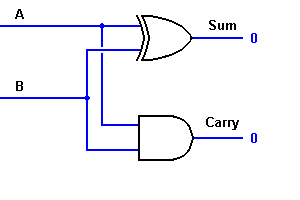
\includegraphics [width=0.5\textwidth] {images/Half-Adder-Circuit}
\end{figure}

A full adder has three inputs, two numbers and a carry-in. It has two
outputs, the sum and carry-out. This setup makes full-adders easy to
chain together. We can implement the full-adder circuit using two
half-adders.

\begin{figure}[hbp]
  \centering
  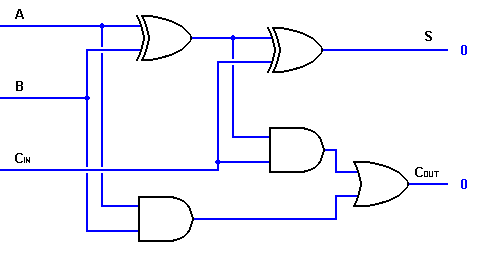
\includegraphics [width=0.7\textwidth] {images/Full-Adder-Circuit}
\end{figure}

\section{Make something cool/useful out of full-adders and
  half-adders. Draw a diagram}

\section{Draw symbols for all the logic gates you can think of.}
\begin{figure}[hbp]
  \centering
  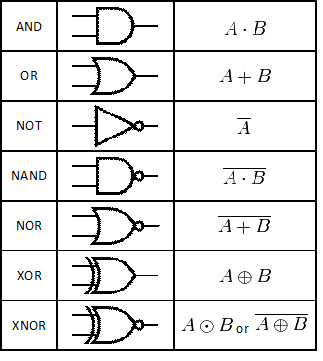
\includegraphics[width=0.5\textwidth] {images/Logic-gates}
\end{figure}

\section{What is sequential logic?}
Sequential logic is a type of logic circuit whose output depends not
only on the present value of its input signals but on the sequence of
past inputs, the input history.

\section{What is combinational logic?}
Combinational logic is a type of digital logic where the output is a
function only of the present inputs.

\section{D flip-flop}
\subsection{What is a D flip-flop?}
The D flip-flop captures the value of the input at a spesific portion
of the clock cycle. The captured value then becomes the output. The
output is held at other parts of the clock cycle.

Truth table

\begin{tabular}{lcr}
  Clock & D & $Q_{next}$ \\ \hline
  Rising edge & 0 & 0 \\
  Rising edge & 1 & 1 \\
  Non-rising & X & Q \\
\end{tabular}

\subsection{Draw the symbol commonly used for representing a D
  flip-flop.}
\begin{figure}[hbp]
  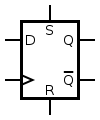
\includegraphics[width=0.3\textwidth]{images/d-flip-flop}
\end{figure}

\subsection{Find VHDL code for a D flip-flop with synchronous reset.}
Here's VHDL code for a single positive edge triggered flip flop with
synchronous reset from the module library.

\lstset{
  language=VHDL,
  basicstyle=\small\sffamily,
  numbers=left,
  numberstyle=\tiny,
  frame=tb,
  columns=fullflexible,
  showstringspaces=false
}

\begin{lstlisting}
library ieee;
use ieee.std_logic_1164.all;
use ieee.numeric_std.all;

entity dff_clr is
  port (
    clk     : in  std_logic;
    reset_n : in  std_logic;
    d       : in  std_logic;
    q       : out std_logic);
end dff_clr;

architecture rtl of dff_clr is
begin
  process(clk, reset_n)
  begin
    if (clk'event and clk='1') then
      if(reset_n = '0') then
        q <= '0';
      else
        q <= d;
      end if;
    end if;
  end process;
end rtl;
\end{lstlisting}

\section{Latch (The evil cousin of the D flip-flop)}
\subsection{What is latch?}
A latch is basically an asynchronous storage element. It has no clock
input. It differs from a flip-flop in that a flip-flop only changes
its output in response to a clock edge. A latch can change its output
in response to some other input regardless of the clock.

\subsection{Try googling ``unwanted latches''.}
There isn't really question here, but unwanted latches is what happens
when there are some outputs that aren't assigned at every branch of
the code. For example if you specify the value in one condition but
not in the other(s). For example,

\begin{lstlisting}
if a = '1' then
   b(0) <= '1';
else
   b(1 downto 0) <= "00";
end if;
\end{lstlisting}

Since the value of b(1) is not specified we would get an unwanted
latch.

\section{What is a register and how are registers related to D
  flip-flops?}
A register is a form of low-level memory. It consists of a flip-flop
for every bit it stores. There are several kinds of registers, but the
simplest one is called a parallel load register.

\section{Draw a 4-bit register}
\begin{figure}[hbp]
  \centering
  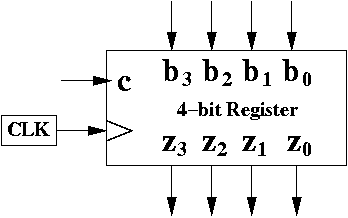
\includegraphics[width=0.3\textwidth]{images/4-bit-register}
\end{figure}

\section{Draw a 4-bit shift-register}
\begin{figure}[hbp]
  \centering
  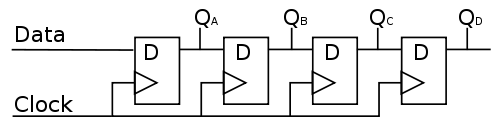
\includegraphics[width=\textwidth]{images/4-Bit-Shift-Register}
\end{figure}

\section{What is a Mux?}
A multiplexer (or mux) is a device that selects one of several input
signals and forwards the selected input into a single line.

\section{Google “CPU datapath”, print out one example Datapath and
  explain what we are looking at.}
A CPU datapath shows how the functional units of a CPU work
together. It typically consists of the program counter, the
instruction register and data-/address memory register.

\begin{figure}[hbp]
  \centering
  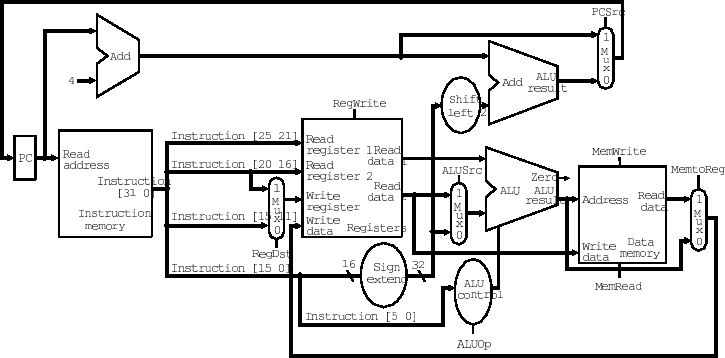
\includegraphics[width=\textwidth]{images/cpu-datapath}
\end{figure}

\section{What is the purpose of pipelining in computing?}
The purpose of pipelining is to increase throughput, typically in
instructions per clock cycle.

\section{What is logic synthesis?}
Logic synthesis is a process by which an abstract form of desired
circuit behavior is turned into a design implementation in terms of
logic gates.

\section{What is high-level synthesis?}
High-level synthesis is an automated design process that interprets an
algorithmic description of a desired behavior and creates digital
hardware that implements that behavior.

\section{What does EDA stand for in the context of digital design?}
EDA stands for Electronic Design Automation.

\section{What does “place \& route” refer to?}
In the context of FPGAs ``place \& route'' refers to the placement and
interconnection of logic elements on the grid of the FPGA.

\section{What is static timing analysis (STA)?}
Static timing analysis (STA) is a simulation method of computing the
expected timing of a digital circuit without requiring a simulation of
the full circuit.

\section{Is negative slack a good thing?}
Negative slack is not a good thing. It implies that a path is too slow
and needs to be sped up if the whole circuit is to work at the desired
speed.

\section{What does ``critical path'' mean?}
Critical path is the slowest logical path in the circuit, and
determines the maximum possible clock rate.

\section{What does the terms ``setup-time'' and ``hold-time'' for a
  flip-flop mean?}
Setup time is the minimum amount of time the data input should be held
steady before the clock event, so that the data is reliably sampled by
the clock.

Hold time is the minimum amount of time the data input should be held
steady after the clock event, so that the data is reliably sampled by
the clock.

\section{What does ``design for testability'' mean?}
Designing for testability means to add testability features to the
product design. The added features make it easier to develop and apply
manufacturing tests to the designed hardware.

\section{What is scan chain?}
Scan chain is a technique used in design for testing.
The objective is to make testing easier by providing a simple way to
set and observe every flip-flop in a circuit.

\section{What is formal verification?}
Formal verification is when you prove or disprove an algorithm using
formal methods of mathematics. It can be helpful in proving the
correctness of systems such as cryptographic protocols and
combinational circuits.

\section{What is a state-machine and what role do they play in digital
circuits?}
A state-machine is a model used to design both computer programs and
sequential logic circuits. A particular state-machine is defined by a
list of its states, its initial state, and the triggering condition
for transition.


\end{document}

%%% Local Variables:
%%% mode: latex
%%% TeX-master: t
%%% End:
